%avoid page number on blank pages when cleared
\thispagestyle{empty}
\cleardoublepage
\chapter{EXPERIMENTOS Y RESULTADOS}
\label{chap:experiments}

%Introduce Chapter: 3 experiments (test set size = 3) to test the whole
%shape matching methodology. Its separated in three main processes: initial
%processing, automatic shape matching and manual fixing. The results are 
%presented and discussed.

En este cap\'itulo se presentan los diferentes experimentos llevados a cabo
para probar el rendimiento de la soluci\'on de detecci\'on y ajuste de formas
desarrollada, explicando la raz\'on de su elecci\'on y los diferentes objetivos
de las pruebas. Seguidamente, se presentan y discuten los resultados obtenidos a
partir de los experimentos, donde se indican las ventajas e inconvenientes 
de la soluci\'on presentada.

\section{Experimentos}
\label{sec:experiments}

Con el objetivo de poner a prueba la soluci\'on implementada, se utilizaron tres im\'agenes
digitales de gusanos en medio l\'iquido, provistas por Johan Henriksson, investigador del
Departamento de Biociencias y Nutrici\'on del Instituto Karolinska en Suecia.\\

A cada imagen le corresponde un nivel de dificultad diferente, asignado de acuerdo a los
al n\'umero de gusanos y grado de solapamiento. As\'i, mientras mayor es la cantidad
de gusanos en la imagen, y mientras mayor es la cantidad de gusanos que se superponen, 
mayor es el nivel de dificultad. El grado de solapamiento se determina por el n\'umero
de gusanos que pertenecen a las diferentes agrupaciones de gusanos, y por la cantidad
de gusanos en la imagen.\\

Las im\'agenes seleccionadas fueron denominadas: \emph{imagen de prueba 1}, \emph{imagen de prueba 2} e
\emph{imagen de prueba 3}. Las caracter\'isticas del conjunto de prueba son mostradas en la tabla \ref{tab:testset}, donde
las diferentes pruebas aparecen en orden creciente de dificultad.


\begin{table}[h]
  \caption{Caracter\'isticas del conjunto de prueba}
\begin{center}
\begin{tabular}[h]{|>{\columncolor[gray]{0.9}} p{2cm} |p{3cm} | p{2.8cm} | p{3cm}| p{2.8cm} |}
    \hline
    \rowcolor[gray]{.9}
    Imagen & N\'umero de Gusanos Aislados & N\'umero de Agrupaciones  & N\'umero de Gusanos en Agrupaciones  & Total de Gusanos\\
    \hline
    Test 1 & 11/19 (57.8\%) & 3 & 8/19 (42.1\%) & 19 \\
    \hline
    Test 2 & 8/33 (24.2\%) & 3 & 25/33 (75.7\%)& 33 \\    
    \hline
    Test 3 & 13/38 (34.2\%)& 5 & 25/38 (65.7\%) & 38 \\
    \hline 
  \end{tabular}
\end{center}
  \label{tab:testset}
\end{table}

Por cada imagen de prueba se llev\'o a cabo una serie de experimentos, para analizar
el rendimiento de los diferentes procesos involucrados en la metodolog\'ia
de la soluci\'on, en base a la implementaci\'on desarrollada. 
El proceso global fu\'e dividido en tres etapas que representan
los pasos fundamentales de la metodolog\'ia: \emph{procesamiento inicial}, 
\emph{detecci\'on y ajuste autom\'atico de formas} y \emph{correci\'on manual}.\\

La etapa de \emph{procesamiento inicial} involucra todos los pasos de procesamiento
de im\'agenes que son realizados antes del proceso de optimizaci\'on, tales como:
segmentaci\'on inicial, transformaci\'on por distancia, \emph{esqueletizaci\'on}, 
agrupamiento de gusanos, detecci\'on de puntos extremos y creaci\'on del perfil de
gusanos. Entre estos, la transformaci\'on por distancia y la \emph{esqueletizaci\'on}
siguen algoritmos previamente analizados y probados, (ver Sec. \ref{sec:metdt} y Sec. \ref{sec:metsk})
y producen resultados sencillos de probar, por lo que no hay necesidad de ahondar en ellos.
El proceso de segmentaci\'on y agrupamiento de gusanos, que se deriva del esqueleto de la
imagen, es igualmente sencillo.\\
Por otro lado, los procesos de segmentaci\'on inicial por un m\'etodo del valor umbral,
detecci\'on de puntos extremos y generaci\'on de perfiles dependen de las caracter\'isticas
de la imagen de entrada, por lo cual se llevaron a cabo diferentes experimentos para analizar
su rendimiento.\\

La etapa de \emph{detecci\'on y ajuste de formas} consiste en un serie de experimentos que tratan
del proceso autom\'atico de optimizaci\'on para ajustar formas en agrupaciones de gusanos y 
gusanos aislados. Estos experimentos buscan medir la eficacia en la detecci\'on y la eficiencia
en tiempo de diferentes variaciones del proceso de ajuste de formas, con el prop\'osito de
sacar conclusiones m\'as detalladas acerca de la eficacia del algoritmo y la factibilidad de
la soluci\'on autom\'atica.\\

La tercera etapa, \emph{correcci\'on manual}, tiene como objetivo medir el tipo y cantidad
de correcciones manuales que deben ser llevadas a cabo por el usuario para corregir 
conformaciones incorrectas, en cada imagen de prueba. Se analiza,
 as\'i mismo, las diferencias entre las diferentes conformaciones factibles por cada
punto extremo, para permitir conclusiones acerca de la sensibilidad del funcional
de energ\'ia.\\

Los experiementos fueron ejecutados en una computadora personal de 2.00 Ghz AMD Turion,
Procesador Mobile Dual-Core, 1MB cache y 3Gb de memoria RAM, bajo Linux, distribuci\'on
Ubuntu.

\section{Resultados}
\label{sec:results}

En esta secci\'on se presentan y discuten los resultados obtenidos de los experimentos
realizados. Los resultados son distribuidos en tres etapas de acuerdo a los experimentos 
llevados a cabo: \emph{procesamiento inicial}, \emph{detecci\'on y ajuste de formas} y 
\emph{correci\'on manual}.

\subsection{Procesamiento Inicial}
\label{sec:initproc}

En esta secci\'on se presentan los resultados de los experimentos llevados a cabo sobre
el conjunto de prueba para los siguientes procesos: segmentaci\'on inicial y detecci\'on
de puntos extremos. Seguidamente, se presenta una breve discusion sobre la generaci\'on
de perfiles de gusanos.

\subsubsection*{Segmentaci\'on Inicial (M\'etodo del Valor Umbral)}

Como se explica en la Sec. \ref{sec:thresimp}, \emph{Endrov} provee implementaciones
para los siguientes MVU: \emph{Fukunaga}, \emph{m\'axima entrop\'ia}, 
\emph{Otsu} y \emph{percentil}. Con la intenci\'on de determinar el m\'etodo m\'as
apropiado, se probaron los diferentes m\'etodos con el conjunto de prueba. La prueba
por m\'etodo consisti\'o, b\'asicamente, en ajustar los par\'ametros 
de entrada hasta encontrar la mejor imagen binaria posible, a partir de cada imagen
del conjunto de prueba.
La determinaci\'on de la calidad de cada imagen binaria se llevo a cab\'o a trav\'es de
inspecci\'on visual.\\

El m\'etodo del valor umbral por percentil result\'o ser el mejor para las tres
im\'agenes del conjunto de prueba, con gran diferencia sobre el resto de los 
m\'etodos. Adem\'as, los mejores valores de percentil por im\'agen resultaron bastante
cercanos entre s\'i, lo que indica la posible factibilidad de ajustar un m\'etodo de valor
umbral autom\'atico para im\'agenes del mismo tipo, que es suceptible de ser desarrollado 
en trabajos futuros. Los mejores valores de percentil por im\'agen son mostrados 
en la Tabla. \ref{tab:threshold}.\\
El m\'etodo de \emph{Fukunaga} produjo resultados aceptables a partir de la combinaci\'on
de im\'agenes binarias generadas con diferentes n\'umero de clases 
(par\'ametro del m\'etodo), sin embargo requiere en general un ajuste m\'as minucioso y 
produjo resultados menos precisos que el m\'etodo de \emph{percentil}.


\begin{table}[h]
  \caption{Mejor valor de percentil para el conjunto de prueba}
\begin{center}
\begin{tabular}[h]{|>{\columncolor[gray]{0.9}} c |c|c|c|}
    \rowcolor[gray]{.9}
    \hline
     & Imagen 1 & Imagen 2 & Imagen 3\\
    \hline
   Percentil & 0.074 & 0.1 & 0.11\\
    \hline
  \end{tabular}
\end{center}
  \label{tab:threshold}
\end{table}

Los mejores valores de percentil oscilaron entre $0.074$ y $0.11$ y fueron sencillos
de determinar utilizando \emph{Endrov}.

\subsubsection*{Detecci\'on de Puntos Extremos}

La tabla \ref{table:endtable} muestra el n\'umero de puntos extremos que 
fueron detectados autom\'aticamente y aquellos que se agregaron de forma
manual, as\'i como el total de puntos extremos de gusanos en la imagen.

\begin{table}[h]
  \caption{Detecci\'on y ajuste de puntos extremos de gusanos en el conjunto de prueba}
\begin{center}
\begin{tabular}[h]{|>{\columncolor[gray]{0.9}} p{3cm} |p{2.9cm}|p{3cm}|p{3.2cm}|}
    \rowcolor[gray]{.9}
    \hline
    Imagen & Total de Puntos Extremos & Puntos Detectados & Puntos Agregados Manualmente\\
    \hline
    Imagen 1 & 38 & 38 (100\%) & 0 \\
    \hline 
    Imagen 2 & 66 & 53 (80\%) & 13 \\
    \hline 
    Imagen 3 & 76 & 57 (75\%) & 19 \\
    \hline
  \end{tabular}
\end{center}
  \label{table:endtable}
\end{table}

En la tabla se puede observar que al existir una gran cantidad de gusanos
que pertenecen a agrupaciones de gusanos, aumenta la probabilidad de que
ocurran solapamiento. De la misma forma, esta probabilidad aumenta 
cuando se presenta una alta densidad de gusanos en la imagen.
Considerando la alta cantidad de gusanos que pertenecen a agrupaciones
de gusanos para la segunda y tercera imagen de prueba, y el bajo
n\'umero de agrupaciones de gusanos (que aumenta el riesgo de solapamiento),
la cantidad de puntos extremos no detectados puede ser considerada 
suficientemente baja, siendo as\'i factible agregarlos a mano.

\subsubsection*{Perfiles de Gusano}

Para generar autom\'aticamente un perfil de gusano preciso y representativo 
de los gusanos de la imagen que se procesa, es necesario que haya presencia
de gusanos aislados. El porcentaje de gusanos aisalados para cada imagen del
conjunto de prueba fueron $57.8\%$, $24.2\%$ y $34.2\%$, respectivamente, 
oscilando entre $8$ y $13$ gusanos por imagen, como se muestra en la tabla
\ref{tab:testset}.\\
Los perfiles de gusanos generados en cada imagen del conjunto de prueba, 
resultaron lo suficientemente representativos como para conducir exit\'osamente
el proceso de optimizaci\'on de ajuste de formas, cuyos resultados son
presentados en las subsecciones de nombre \emph{ajuste autom\'atico de formas},
mostradas m\'as adelante.

\subsection{Detecci\'on y Ajuste de Formas}

En esta secci\'on se presentan los resultados de la segunda y tercera
etapa general de la metodolog\'ia de la soluci\'on, para cada imagen de prueba.
Estas etapas consisten en el \emph{detecci\'on y ajuste autom\'atico de formas} y en los procesos 
de \emph{correcci\'on manual}, tal como fueron descritas en la Sec. \ref{sec:experiments}.\\

En la secci\'on de \emph{detecci\'on y ajuste autom\'atico de formas} se presentan los resultados
para cuatro variantes del algoritmo de detecci\'on y ajuste de formas, diferenciando
la precisi\'on del ajuste y el rendimiento en tiempo. Las dos variantes principales
son denominanadas: \emph{predicci\'on} y \emph{multicamino}.\\
\emph{Predicci\'on}, es una versi\'on del algoritmo en la cual se toman en cuenta 
los caminos calculados a trav\'es del algoritmo de predicci\'on de caminos, presentado
en la Sec. \ref{sec:pathguessing}. Los caminos m\'as probables que parten de cada punto
extremo son favorecidos, disminuyendo por un factor el valor de distancia de las
conformaciones encontradas a partir de estos caminos, de manera que aumente la 
probabilidad de ser escogidos en la asignaci\'on final. Por su parte, la variante 
\emph{multicamino} no favorece a los caminos inducidos por predicci\'on, y toma 
en cuenta todos los caminos posibles.\\
Cada variante es probada agregando y sin agregar los puntos extremos faltantes, lo
que consituye las cuatro variantes mencionadas inicialmente.\\

La secci\'on de \emph{correcci\'on manual} presenta los resultados obtenidos 
al llevar a cabo la modificaci\'on manual de las conformaciones incorrectas.
Por cada prueba, se muestran la imagen resultante del ajuste autom\'atico, 
y la imagen resultante de la correcci\'on, donde se resaltan las conformaciones
que fueron corregidas. Este proceso es llevado a cabo manualmente: el usuario
detecta una conformaci\'on incorrecta visualmente y, seguidamente, selecciona el
par de puntos extremos correctos para obtener la mejor conformaci\'on
calculada a partir de un camino que conecta dichos puntos, 
tal como se explica en la Sec. \ref{sec:matchfix}.\\
Una operaci\'on (de la forma en que se utiliza en las tablas de esta secci\'on)
se considera como la acci\'on de seleccionar dos puntos extremos y generar
una nueva conformaci\'on.\\

Seguidamente, se presenta la secci\'on \emph{optimizaci\'on de energ\'ia}, en la que
se presenta y se discute la distribuci\'on de los valores de energ\'ia para las diferentes 
conformaciones, por cada imagen de prueba. 

\subsubsection*{Detecci\'on y Ajuste Autom\'atico (Imagen de Prueba 1)}

Dado que todos los puntos extremos de la \emph{imagen 1} son encontrados
autom\'aticamente, como se muestra en la Tabla \ref{table:endtable}, solo
se presentan los resultados para las variantes \emph{multicamino} y \emph{predicci\'on},
que incluyen todos los puntos extremos. La efectividad de detecci\'on y el tiempo
de corrida para estas variantes son presentadas en la Tabla \ref{table:auto1}.

\begin{table}[h!]
  \caption{Resultados del ajuste autom\'atico de gusanos en la imagen 1}
  \begin{center}
  \begin{tabular}{|>{\columncolor[gray]{0.9}} p{3cm}|p{2.8cm}|p{2.8cm}|p{2.8cm}|c|}
    \hline
    \rowcolor[gray]{.9}
    Variante & Gusanos aislados ajustados & Gusanos ajustados en agrupaciones 
    & Ajuste Total
    & Tiempo (s) \\ 
    \hline
    Multicamino & 11/11 (100\%) & 6/8 (75\%) & 17/19 (89.5\%)& 6.47 \\
    \hline
    Predicci\'on & 11/11 (100\%) & 8/8 (100\%) & 19/19 (100\%) & 7.53 \\
    \hline
  \end{tabular}
\end{center}
  \label{table:auto1}
\end{table}

Se puede observar que para ambas variantes los gusanos aislados
fueron detectados en su totalidad. Para la variante \emph{multicamino}
se ajustaron correctamente tres cuartos de los gusanos en agrupaciones.
Por otro lado, la variante \emph{predicci\'on} permiti\'o ajustar correctamente
todos los gusanos de la imagen, de forma autom\'atica. El tiempo de ejecuci\'on
es ligeramente mayor para la variante de \emph{predicci\'on}, como era de esperarse 
debido a los c\'alculos adicionales requeridos por el algoritmo de predicci\'on
de caminos.\\

Para esta imagen, la variante \emph{predicci\'on} present\'o una mejora considerable
a la soluci\'on, al inducir la selecci\'on de caminos m\'as probables. Por otro lado,
los gusanos aislados fueron detectados en su totalidad, independientemente
de la variante seguida. La asignaci\'on de conformaciones de la variante \emph{predicci\'on}, 
para la \emph{imagen 1}, es mostrada en la Fig. \ref{fig:best1}.

\begin{figure}[h!]
  \centering
  \subfloat[Best match]{\label{best1}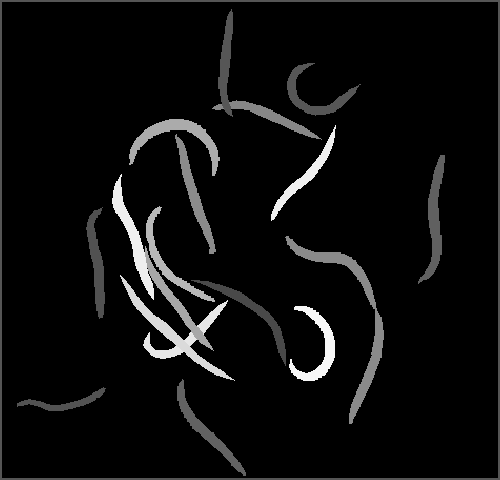
\includegraphics[scale=0.34]{results/test1/complete-frame1}}
\qquad
  \subfloat[Best match over original image]{\label{bestbg1}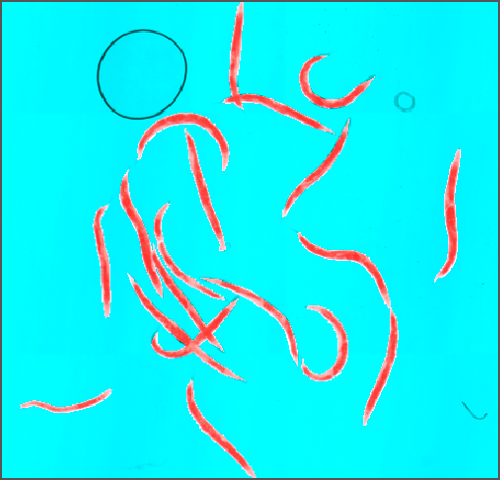
\includegraphics[scale=0.34]{results/test1/complete-framebg1}}
  \caption{Mejor ajuste autom\'atico en la imagen 1}
  \label{fig:best1}
\end{figure}

\subsubsection*{Detecci\'on y Ajuste Autom\'atico (Imagen de Prueba 2)}

En la tabla \ref{tab:tab2} se muestran los resultados del proceso de detecci\'on y
 ajuste autom\'atico de formas, para la \emph{imagen 2}.

\begin{table}[h]
 \caption[Resultados del ajuste autom\'atico de gusanos en la imagen 2]{Resultados del ajuste autom\'atico de gusanos en la imagen 2, agregando y sin agregar puntos extremos faltantes (pf)}
\begin{tabular}{|>{\columncolor[gray]{0.9}} p{3.2cm}|p{2.8cm}|p{2.8cm}|p{2.8cm}|c|}
    \hline
    \rowcolor[gray]{.9}
    Variante & Gusanos aislados ajustados & Gusanos ajustados en agrupaciones 
    & Ajuste Total
    & Tiempo (s) \\     
    \hline  
    Multicamino - pf & 8/8 (100\%) & 7/25 (28\%) & 15/33 (45.4\%) & 21.8 \\ 
    \hline
    Predicci\'on - pf & 8/8 (100\%) & 10/25 (40\%) & 18/33 (54.5\%) & 23.7\\
    \hline
    Multicamino + pf & 8/8 (100\%)& 15/23 (65.2\%) & 23/33 (69.7\%)& 42.3 \\
    \hline
    Predicci\'on + pf & 8/8 (100\%)& 21/25 (84\%) & 29/33 (87.8\%) & 45 \\
    \hline
  \end{tabular}
  \label{tab:tab2}
\end{table}

Se puede observar que la totalidad de gusanos aislados fue detectada
en cada variante. Para las dos variantes con puntos extremos faltantes,
solo se pudo ajustar correctamente alrededor de la mitad de los gusanos
en la imagen. Aqu\'i se evidencia el hecho de que la falta de un punto 
de extremo determinado hace imposible detectar el gusano al que corresponde.\\

Para las variantes que incluyen los puntos extremos, los resultados son
considerablemente superiores. Se puede observar que en las variantes de 
\emph{predicci\'on} mejora la precisi\'on de detecci\'on, tanto cuando
se incluyen los puntos extremos faltantes como cuando no se incluyen. As\'i
mismo, el tiempo de ejecuci\'on aumenta cuando los puntos extremos son
agregados, como es de esperarse.\\
Para la variante de \emph{predicci\'on} el porcentaje de ajuste es
considerablemente m\'as alto que para la variante de \emph{multicamino}.
En el mejor de los casos, el proceso autom\'atico permite ajustar
la forma de todos los gusanos aislados y un alto porcentaje de los
gusanos que pertenecen a agrupaciones ($87.8\%$), en menos de un minuto.

\subsubsection*{Correcion Manual (Imagen de Prueba 2)}

La variante de \emph{predicci\'on} sin puntos faltantes dio los mejores
resultados con solo cuatro gusanos aislados ajustados incorrectamente, sobre
un total de treinta y tres. La F\'igura \ref{fig:best2} muestra una comparaci\'on de 
las conformaciones encontradas de manera autom\'atica y 
las conformaciones corregidas de forma manual.

\begin{figure}[h]
  \centering
  \subfloat[Ajuste autom\'atico]{\label{test2:best2}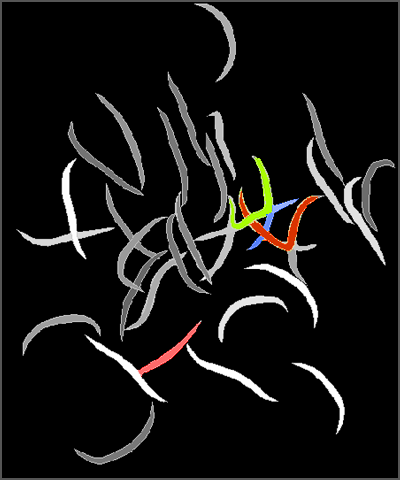
\includegraphics[scale=0.45]{results/test2/guessing-nobgframe}}
\qquad
  \subfloat[Ajuste autom\'atico superpuesto con imagen original]{\label{bestbg1}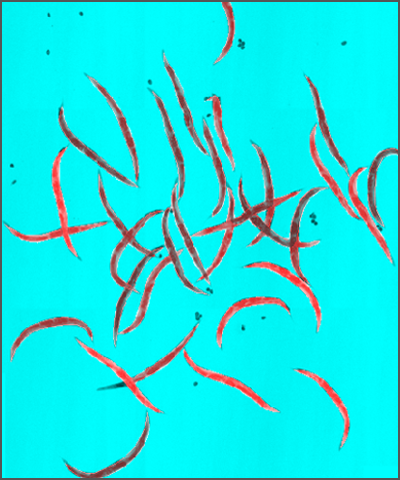
\includegraphics[scale=0.45]{results/test2/guessing-bgframe}}
\qquad
  \subfloat[Ajuste autom\'atico y manual]{\label{test2:bestbg2}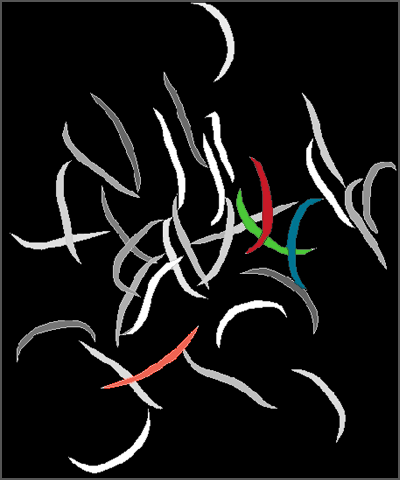
\includegraphics[scale=0.45]{results/test2/frame2-allnobg}}
\qquad
  \subfloat[Ajuste autom\'atico y manual superpuesto con imagen original]{\label{bestbg1}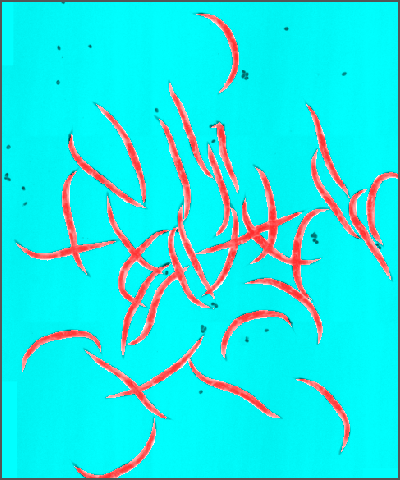
\includegraphics[scale=0.45]{results/test2/frame2-all}}

\caption[Mejor ajuste autom\'atico y correcci\'on manual en la imagen 2]{Mejor ajuste autom\'atico y correcci\'on manual en la imagen 2.
Las formas y contornos en color en im\'agenes \ref{test2:best2} y \ref{test2:bestbg2} indican gusanos detectados incorrectamente} 
\label{fig:best2}
\end{figure}

A trav\'es del proceso manual se pudieron corregir todas las conformaciones asignadas incorrectamente.
De esta manera se pudo detectar y ajustar la forma de todos los gusanos de la imagen.

\subsubsection*{Correcci\'on Manual (Imagen de Prueba 3)}

Los resultados del proceso de detecci\'on y ajuste autom\'atico de formas en 
la \emph{imagen 3} son presentados en la Tabla \ref{tab:tab3}. 


\begin{table}[h!]
 \caption[Resultados del ajuste autom\'atico de gusanos en la imagen 3]{Resultados del ajuste autom\'atico de gusanos en la imagen 3, agregando y sin agregar puntos extremos faltantes (pf)}
\begin{tabular}{|>{\columncolor[gray]{0.9}} p{3.2cm}|p{2.8cm}|p{2.8cm}|p{2.8cm}|c|}
    \hline
    \rowcolor[gray]{.9}
    Variante & Gusanos aislados ajustados & Gusanos ajustados en agrupaciones 
    & Ajuste Total
    & Tiempo (s) \\     
    \hline  
    Multicamino - pf & 13/13 (100\%) & 5/25 (20\%) & 18/38 (47.3\%) & 26.4 \\ 
    \hline
    Predicci\'on - pf & 13/13 (100\%) & 7/25 (28\%) & 20/38 (52.6\%) & 28.7\\
    \hline
    Multicamino + pf & 13/13 (100\%)& 13/25 (52\%) & 26/38 (68.4\%)& 36.2 \\
    \hline
    Predicci\'on + pf & 13/13 (100\%)& 16/25 (64\%) & 29/38 (76.3\%) & 39.8 \\
    \hline
  \end{tabular}
  \label{tab:tab3}
\end{table}

Los gusanos aislados fueron detectados en su totalidad.
Para las variantes de \emph{predicci\'on} y \emph{multicamino} con
puntos extremos faltantes, el porcentaje de detecci\'on se ubica
alrededor de la mitad de los gusanos la imagen. Por el contrario,
en las variantes que incluyen los puntos extremos faltantes, el nivel
de precisi\'on aumenta considerable.
La variante de \emph{predicci\'on} es siempre mejor que \emph{multicamino}, 
aunque un poco m\'as lenta. La mejor variante result\'o ser \emph{predicci\'on} sin
puntos faltantes, alcanzando a ajustar correctamente todos los gusanos aislados y
un total de tres cuartos de la imagen total.

\subsubsection*{Correcci\'on Manual (Imagen de Prueba 3)}

La variante de \emph{predicci\'on} que incluye los puntos faltantes result\'o ser la mejor, donde solo nueve gusanos
fueron detectados incorrectamente sobre un total de treinta y ocho. La Figura \ref{fig:best3} 
muestra una comparaci\'on de las conformaciones encontradas de manera autom\'atica y 
las conformaciones corregidas de forma manual.

\begin{figure}[h!]
  \centering
  \subfloat[Ajuste autom\'atico]{\label{test3:best3}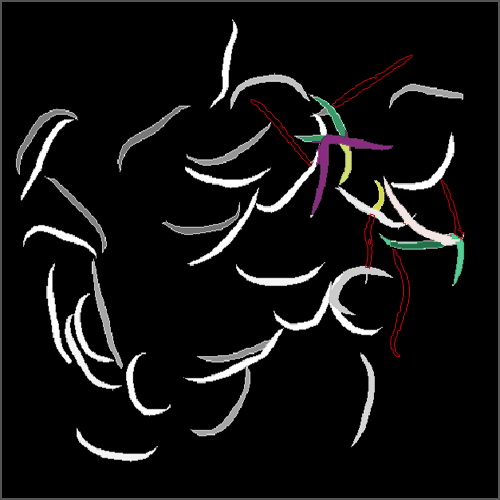
\includegraphics[scale=0.35]{results/test3/guess-nobg}}
\qquad
  \subfloat[Ajuste autom\'atico superpuesto con imagen original]{\label{bestbg1}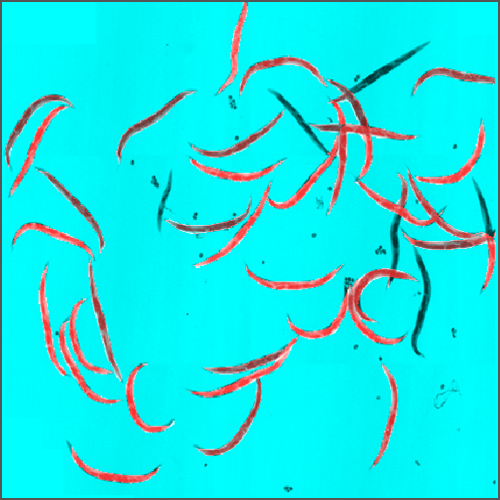
\includegraphics[scale=0.35]{results/test3/guess-bg}}
\qquad
  \subfloat[Ajuste autom\'atico y manual]{\label{test3:bestbg3}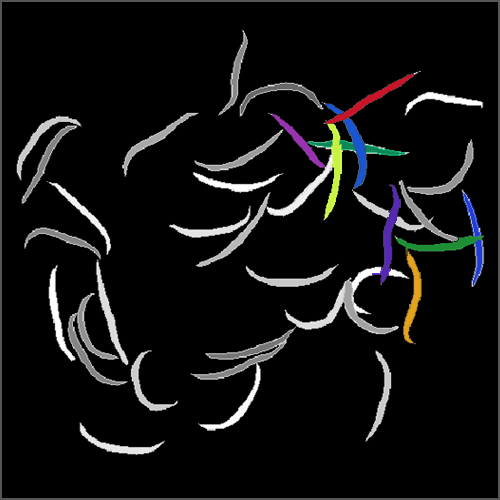
\includegraphics[scale=0.35]{results/test3/all-nobg}}
  \label{best3:c}
\qquad
  \subfloat[Ajuste autom\'atico y manual superpuesto con imagen original]{\label{bestbg1}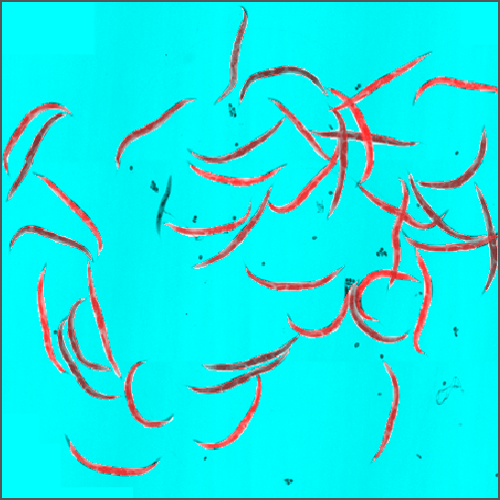
\includegraphics[scale=0.35]{results/test3/all-bg}}
\caption[Mejor ajuste autom\'atico y correcci\'on manual en la imagen 3]{Mejor ajuste autom\'atico y correcci\'on manual en la imagen 3.
Las formas y contornos en color en im\'agenes \ref{test3:best3} y \ref{test3:bestbg3} indican gusanos detectados incorrectamente} 
 \end{figure}

Se requirieron nueve operaciones simples para corregir los gusanos ajustados
incorrectamente. Todos los gusanos en la imagen pudieron ser detectados
y ajustados.

\subsection{Optimizaci\'on de Energ\'ia}

El valor de energ\'ia de una conformaci\'on determina su grado de precisi\'on
con respecto a la f\'igura. Tal como se describe en la Sec. \ref{sec:energyformulation},
la funci\'on de energ\'ia eval\'ua la distancia entre formas como el porcentaje
de p\'ixeles de fondo que estan contenidos en la silueta que se ajusta, por lo que
todos los posibles valores de energ\'ia estan contenidos en el intervalo $[0,1]$.\\

En la Figura \ref{fig:energy123} se muestran los valores de energ\'ia para las mejores
tres conformaciones por cada punto extremo de gusano. La primera corresponde a la 
conformaci\'on correcta y ajusta el gusano de la imagen. Las siguientes dos
corresponden a las mejores conformaciones entre puntos extremos incorrectos. 
Estas \'ultimas dos seran denominadas primera conformaci\'on incorrecta y 
segunda conformaci\'on incorrecta, respectivamente.

\captionsetup[subfloat]{farskip=-0.8cm,captionskip=-0.2cm}
%Distance between images could be reduced to make graphs larger
\begin{figure}[htp]
  \begin{center}
    \subfloat[Imagen 1]{\label{fig:energy1b}\includegraphics[scale=0.54]{results/test1/energy-graph}}\\
    \subfloat[Imagen 2]{\label{fig:energy2b}\includegraphics[scale=0.54]{results/test2/energy-graph}}\\
    \subfloat[Imagen 3]{\label{fig:energy3b}\includegraphics[scale=0.54]{results/test3/energy-graph}}
  \end{center}
  \caption[Valor de energ\'ia de las tres mejores conformaciones por punto extremo en el conjunto de prueba]
  {Valor de energ\'ia de las mejores tres conformaciones por punto extremo en el conjunto de prueba.
    Los puntos extremos corresponden a gusanos en agrupaciones con m\'as de dos conformaciones posibles}
  \label{fig:energy123}
\end{figure}
\showcaptionsetup{subfloat}

\subsubsection*{Image de Prueba 1}

Para la mayor\'ia de los puntos extremos la conformaci\'on correcta 
tiene el menor valor de energ\'ia.
En solo dos casos, existe una conformaci\'on incorrecta que tiene un valor
de energ\'ia menor. La segunda conformaci\'on incorrecta posee siempre
un valor de energ\'ia mayor que la conformaci\'on correcta.

\subsubsection*{Imagen de Prueba 2}

Se puede observar que la segunda conformaci\'on incorrecta (en verde) es,
en todos los casos, bastante peor que la conformaci\'on correcta. Por esto,
la conformaci\'on correcta corresponde siempre a la mejor o a segunda mejor
conformaci\'on encontrada, en t\'erminos de energ\'ia, de todas las posibles.
Para esta imagen, solo en cuatro de veintinueve puntos extremos se
sit\'ua a la primera conformaci\'on incorrecta (en rojo) con un mejor valor de
energ\'ia que la correcta (en azul). Esto coincide con los 
resultados mostrados en la Tabla \ref{tab:tab3}, donde, para la mejor
variante autom\'atica, la cantidad de gusanos ajustados correctamente
fue de veintinueve, sobre un total de treinta y tres, indicando error
en cuatro puntos extremos (la misma cantidad de puntos en los cuales
la conformaci\'on correcta no tuvo el mejor valor de energ\'ia). 
As\'i mismo, la diferencia de energ\'ia entre la conformaci\'on
correcta y la primera incorrecta, para estos cuatro puntos, es lo
suficientemente peque\~na para pensar que una funci\'on objetivo m\'as sensitiva
podr\'ia permitir calcular la conformaci\'on correcta en todos los casos,
de manera autom\'atica.
 
\subsubsection*{Image de Prueba 3}

Solo para nueve de los veintidos puntos extremos, la primera conformaci\'on
incorrecta result\'o tener un mejor valor que la conformaci\'on correcta.
Esto coincide con los resultados presentados en la Tabla \ref{tab:tab3},
donde, para la mejor variante, la cantidad de gusanos detectados incorrectamente
fue tambien de nueve, an\'alogamente al caso anterior.\\
Para cada punto extremo, con la excepci\'on de uno, la segunda conformaci\'on
incorrecta presenta un valor de energ\'ia menor a la conformaci\'on correcta.
Por lo que la conformaci\'on correcta se encuentra siempre
entre las mejores dos, entre todas las conformaciones calculadas.\\

Dado que para esta imagen la cantidad de gusanos que pertenecen a agrupaciones
de gusanos es alta (25), la probabilidad de conformaciones
incorrectas aumenta. Se obtuvo una alta cantidad de conformaciones correctas 
que no obtuvieron el mejor valor de energ\'ia, se pudiera inferir que la funci\'on de distancia
no es lo suficientemente expresiva. Sin embargo, las diferencias entre la
conformaciones correctas y las seleccionadas para estos casos son estrechas
(al igual que para la \emph{imagen 2}), por lo que una funci\'on objetivo
m\'as sofisticada podr\'ia conducir a mejores resultados.
